\documentclass[a4paper, 10pt]{article}

% % Defining Times Fonts (more compact)
% \renewcommand{\sfdefault}{phv}
% \renewcommand{\rmdefault}{ptm}
% \renewcommand{\ttdefault}{pcr}

%% Particular packages (insert here any packages you want)
\usepackage{amsfonts,amssymb,amsmath,amsthm}
\usepackage{subfigure}
\usepackage{graphicx}
\graphicspath{{figures/}{../Biblio/}}
\usepackage[footnotesize]{caption}
\usepackage[utf8]{inputenc} %Manage accents (useful when writing things in French)
\usepackage[numbers]{natbib}
\usepackage{hyperref}
\usepackage{array, multirow, multicol}
\usepackage{bm}
\usepackage{dsfont}

% Scheme
\usepackage{tikz}
\usetikzlibrary{arrows}
\usetikzlibrary{positioning}

%% Custom math operators
\DeclareMathOperator*{\argmin}{arg\,min\,}
\DeclareMathOperator*{\prox}{prox}
\DeclareMathOperator*{\divergence}{div}
\DeclareMathOperator*{\mini}{min}
\DeclareMathOperator*{\sign}{sign}

%% The page style must be empty (we will add page numbers in the final proceedings)
\renewcommand{\thepage}{}
% Remark: Command \pagestyle{empty} does not delete the the first page number

%% Please dont touch this size commands
%% Set a margin of 15mm from each edge of the paper
\usepackage[top=1.5cm, left=1.5cm, right=1.5cm, bottom=1.5cm]{geometry}

%% Title
\title{
\begin{center}
The mathematics of one-step spectral CT reconstruction methods, one step at a time
\end{center}
}

%% Order author name and affiliation simply like this
\author{Cyril Mory, Simon Rit \& Bruno Sixou}
\date{11 January 2018} % no need for a date

% %% Redefining abstract default style in the article template
% \renewenvironment{abstract}{\bf\small {\em\ Abstract---}}{}


\begin{document}

\maketitle

\begin{abstract}
5 papers, redoing all the maths with many more intermediate steps than in the original papers,
and correcting the mistakes hidden in them.
Then implementation in a lightweight matlab framework, and comparisons
\end{abstract}

\section{Introduction}
Each section starts with the notations of the paper. These are defined throughout the original papers as the calculations
are presented, but having them all available in a single place helps a great deal when trying to re-do the calculations.

\section{Synthetic material basis: mu-preconditioning}
\label{sec:mu}
Section 3.4 of \cite{barber_algorithm_2016} proposes to modify the material attenuation matrix $\mu$ to speed up and stabilize the internal computations.
They call this step ``$\mu$-preconditioning'', but it can be interpreted as generating a basis of synthetic materials instead of the original materials.
These synthetic materials are linear combinations of the original ones, possibly with negative coefficients. We present three ways to choose this basis, i.e.
three different $\mu$-preconditionings. Each one provides a matrix $P$ such that $ \mu_{\text{real}} P = \mu_{\text{synth}}$:
\begin{itemize}
 \item Normalizing $\mu_{\text{real}}$: each column of $\mu_{\text{real}}$ is divided by its norm. This has the advantage of not introducing negative attenuations. 
 The added complexity associated with the use of negative attenuation coefficients, like the use of absolute values in the calculation of 
 $\Sigma^{(n)}$ and $T^{(n)}$ in \cite{barber_algorithm_2016}, can be avoided with this synthetic materials basis
 \item Orthonormalizing $\mu_{\text{real}}$: either using the Gram-Schmidt algorithm or diagonalizing $\mu_{\text{real}}^T \mu_{\text{real}}$ (as proposed in \cite{barber_algorithm_2016}), the column of $\mu_{\text{real}}$ are made 
 orthogonal to each other, in addition to being normalized. This will generate negative attenuation coefficients (for the dot products between columns to be zero)
 \item Computing
 \begin{equation*}
  Q = \frac{S \mu_{\text{real}}}{S \mathds{1}} \quad \text{i.e.} \quad \left( Q \right)_{b,m} = \frac{\sum_e S_{b,e} \mu_{\text{real} \quad e,m}}{\sum_e S_{b,e}}
 \end{equation*}
with $S_{b,e}$ the effective spectrum at energy $e$ in bin $b$, and $\mu_{\text{real} \quad e,m}$ the attenuation of material $m$ at energy $e$.
Each value $\left( Q \right)_{b,m} $ is a weighted mean of the attenuation coefficients of material $m$ over the whole energy spectrum, 
the weights being the number of photons seen by the detector in bin $b$. Roughly, it evaluates how much the material $m$ attenuates
the photons that will end up being detected in bin $b$. 
Now, the problem of determining which linear combination of materials causes the observed attenuation would be much easier 
if each material attenuated the photons of only one bin, i.e. if $Q$ was diagonal. Therefore, we multiply $\mu$ by the inverse of $Q$, which we denote $P$.
When $Q$ is not square, e.g. when there are more bins that materials, $Q$ cannot be inverted, but $P$ can be defined as the Moore-Penrose pseudo inverse of $Q$, i.e.
$P = (Q^TQ)^{-1}Q^T$, which provides a good replacement for $Q^{-1}$. This approach was proposed in \cite{fessler_method_2003} for dual energy CT,
but its extension to more materials and more bins is straightforward.
The basis created this way has as many synthetic materials as the number of bins, each of which can have negative attenuation coefficients.
\end{itemize}

\section{Cai et al. 2013}
The paper \cite{cai_full-spectral_2013} was originally designed for dual-energy CT with fast kV-switching. Therefore, in the paper, each 
pixel of the measured data is assumed to contain two values, one for each tube voltage, indexed by $u$. We adapt the proposed method to spectral CT.
$u$ is now used to index the energy bin number. We focus on the discrete model and discard the notations of the continuous model given
at the beginning of the paper. 

\subsection{Notations and intermediate variables}
\begin{itemize}
  \item $u \in \left\lbrace1..N_v\right\rbrace$: index of energy bin
  \item K: total number of pixels, i.e. number of projections $\times$ number of pixels in one projection
  \item $\varepsilon \in \left\lbrace1..N_\varepsilon \right\rbrace$: actual energy of a photon
  \item $s(u,\varepsilon)$: normalized effective spectrum, i.e. ratio between the number of counts in bin $u$ 
  caused by photons of actual energy $\varepsilon$ without object, and the total number of counts in bin $u$ without object
  \item $\bar{y}(\pmb{t},u)$: expected beam transmission ratio in pixel $\pmb{t}$ and bin $u$, i.e. expected ratio between the number of
  counts with object and without object
  \item $N$: number of voxels in a single material volume
  \item $m \in \left\lbrace1..n_f \right\rbrace$: index of basis material
  \item $x$: column vector for the object volume. First the volume for material 1, then for material 2, etc...
  \item $A$: forward projection matrix for a single material volume
  \item $R$: block-diagonal matrix, $n_f$ blocks, each block is a matrix $A$
  \item $M_1$: matrix of material attenuations. Each column of the matrix $M_1$ is a vector (of height $N_\varepsilon$) 
  containing the attenuation of one material as a function of energy
  \item $M$: large matrix, obtained by replacing each value of $M_1$ by its product with $I_K$, the identity matrix of size $K$
  \item $B=MR$: matrix performing forward projection and computing linear combination with material attenuations.
  $N \times n_f$ columns and $K \times N_\varepsilon$ rows. Thus, $Bx$ is a column vector of size $K \times N_\varepsilon$, 
  i.e. one volume per energy
  \item $S_1$: normalized effective spectrum matrix. One row per bin, one column per energy. Each row sums to 1
  \item $S$: large matrix, obtained by replacing each value of $S_1$ by its product with $I_K$
  \item $\bar{y} = S \exp(-Bx)$: column vector of expected beam transmission ratios, of size $K \times N_v$
\end{itemize}

\subsection{Step by step calculations}
The authors assume that the variance $\theta_1$ of the measured beam transmission ratios $\bar{y}$ can be known. 
They also assume a prior on $x$ which results in minimizing the Huber function of the spatial gradient, which
is close to the behaviour of anisotropic TV minimization. 
The dependencies between variables can be summarized in the diagram shown in figure \ref{fig:dependenciesDiagram}.
\begin{figure}
 \begin{center}
 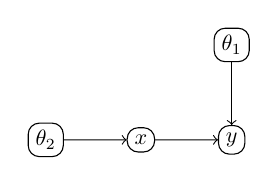
\begin{tikzpicture}[scale=0.8,transform shape]
 \begin{scope}[every node/.style={draw,rectangle, rounded corners}]
 \node (a) {$\theta_1$};
 \node [below =of a] (b){$y$};
 \node [left =of b] (c) {$x$};
 \node [left =of c] (d) {$\theta_2$};
 \end{scope}
 \draw [->] (a) -- (b);
 \draw [->] (c) -- (b);
 \draw [->] (d) -- (c);
 \end{tikzpicture}
 \end{center}
 \caption{Dependencies between variables in Cai2013}
 \label{fig:dependenciesDiagram}
\end{figure}
%
From this diagram, the following expression of the full joint probability can be inferred:
\begin{equation*}
  p(x,y,\theta_1, \theta_2) = p(\theta_1) p(\theta_2) p(x | \theta_2) p(y | x, \theta_1)
\end{equation*}
A basic property of the conditional probabilities also gives
\begin{equation*}
 \begin{split}
  p(x,y,\theta_1, \theta_2) &= p(x,\theta_1 |y,\theta_2) p(y, \theta_2) \\
			    &= p(x,\theta_1 |y,\theta_2) p(y | \theta_2) p(\theta_2)
 \end{split}
\end{equation*}
%
Therefore, equating the right hand sides, we have
\begin{equation*}
 \begin{split}
  p(x,\theta_1 |y,\theta_2) p(y | \theta_2) p(\theta_2) &= p(\theta_1) p(\theta_2) p(x | \theta_2) p(y | x, \theta_1)
 \end{split}
\end{equation*}
Simplifying $p(\theta_2)$ and moving $p(y | \theta_2)$ yields equation (20) of \cite{cai_full-spectral_2013}.
Along equations (21) to (24), the authors assume that $\theta_1$, the variance of $y$, is proportional to $y$.
If $\bar{y}$ is a sufficiently good estimate of $y$, $\theta_1$ is then also proportional to $\bar{y}$. 
They note the proportionality factor $k_d$. It depends on the detector, and can be obtained by calibration.
Let us continue with equation (25):
\begin{equation*}
 \hat{x} = \argmin\limits_x \left\lbrace -\log \left[ p(y | x, \hat{\theta_1})\right] - \log \left[ p(x|\theta_2)\right] \right\rbrace
\end{equation*}
Replacing both probabilities from equations (14) and (17):
\begin{equation*}
 \begin{split}
 \hat{x} &= \argmin\limits_x \left\lbrace -\log \prod_{j=1}^{KN_v} \frac{1}{\sqrt{2\pi \sigma_j^2}} \exp \left\lbrace - \frac{(y_j - \bar{y}_j)^2}{2 \sigma_j^2} \right\rbrace + \Phi(Dx,\theta_2) \right\rbrace \\
 &= \argmin\limits_x \left\lbrace \sum_{j=1}^{KN_v} \left[ \frac{(y_j - \bar{y}_j)^2}{2 \sigma_j^2} - \log \left( \frac{1}{\sqrt{2\pi \sigma_j^2}} \right) \right] + \Phi(Dx,\theta_2) \right\rbrace
 \end{split}
\end{equation*}
From equation (24), $\sigma_j^2 = k_d \bar{y}_j$, therefore
\begin{equation*}
 \hat{x} = \argmin\limits_x \left\lbrace \sum_{j=1}^{KN_v} \left[ \frac{(y_j - \bar{y}_j)^2}{2 k_d \bar{y}_j} + \frac{1}{2} \log 2\pi k_d + \frac{1}{2} \log \left( \bar{y}_j \right) \right] + \Phi(Dx,\theta_2) \right\rbrace
\end{equation*}
Removing the term constant with $x$, multiplying by 2 and cutting the sum into two parts, we obtain
\begin{equation*}
 \hat{x} = \argmin\limits_x \left\lbrace \sum_{j=1}^{KN_v} \frac{(y_j - \bar{y}_j)^2}{k_d \bar{y}_j} + \sum_{j=1}^{KN_v} \log \left( \bar{y}_j \right) + 2 \Phi(Dx,\theta_2) \right\rbrace
\end{equation*}
The first sum can be compactly written in matrix form. In fact, it is exactly a weighted least squares expression, with weights equal to the inverse of the variance of the measurements. 
Doing that yields equation (27).

The algorithm employed to minimize the cost function $J$ is a non-linear conjugate gradient. Equations (28) and (29) are standard, 
the originality here is the choice of the step length $\alpha^{(k)}$, which is explained quite clearly in the paper. In equations (30) and (31), all coefficients of the second degree polynomial in
$\alpha$ are scalars, so the calculation is straightforward. The only difficulty is to actually compute $g$ and $d^THd$. This is done in the appendix.
Note that there is a sign error in equation (32). The appendix contains the correct expression of $g$.

\subsection{Modifications for synthetic materials}
\label{sec:modifs}
In the case where the algorithm is fed a matrix $M_{\text{synth}}$ of the attenuations of synthetic materials, obtained by linear combination of the attenuations of real materials (the columns of $M_{\text{real}}$), 
it will reconstruction synthetic material volumes $x_{\text{synth}}$. The expression for the data-attachment term remains correct, but the regularization must be perfomed on the real materials volumes $x_{\text{real}}$,
since we want the real material volumes to be regular, not the synthetic ones. To clarify the link between $M_{\text{real}}$, $M_{\text{synth}}$, $x_{\text{real}}$ and $x_{\text{synth}}$, let us first imagine that our volumes
are made of a single voxel. Let us also note that the total attenuation coefficient for each energy through that volume should be the same, whether we use synthetic or real materials. This condition gives us 
the following identity:
\begin{equation*}
 M_{\text{real}} x_{\text{real}} = M_{\text{synth}} x_{\text{synth}}
\end{equation*}
Let $P$ be the matrix such that $ M_{\text{real}} P = M_{\text{synth}}$. Then
\begin{equation*}
  \begin{split}
  & M_{\text{real}} x_{\text{real}} = M_{\text{real}} P x_{\text{synth}} \\
  \iff & M_{\text{real}} \left( x_{\text{real}} - P x_{\text{synth}} \right) = 0
  \end{split}
\end{equation*}
Since the columns of $M_{\text{real}}$ are linearly independent by construction (the materials are chosen to have independant attenuation curves), this means $x_{\text{real}} = P x_{\text{synth}}$.
So the same matrix is used to transform the real attenuation matrix into the synthetic one and, the other way round, to transform the synthetic volumes into the real ones. 
In order to apply regularization on real materials, the regularization term $J_2$, its gradient $g_2$ and its Hessian $H_2$ must be replaced by their counterparts adapted to synthetic materials 
$\widetilde{J}_2$, $\widetilde{g}_2$ and $\widetilde{H}_2$ defined as follows:
\begin{equation*}
 \begin{split}
 \widetilde{J}_2(x_{\text{synth}}) &= J_2(P x_{\text{synth}}) = 2 \Phi(Dx_{\text{real}},\theta_2) \\
 \widetilde{g}_2(x_{\text{synth}}) &= P^T g_2(P x_{\text{synth}}) = 2 P^T D^T \dot{\Phi}(Dx_{\text{real}},\theta_2) \\
 \widetilde{H}_2(x_{\text{synth}}) &= P^T H_2(P x_{\text{synth}}) P = 2 P^T D^T \ddot{\Phi}(Dx_{\text{real}},\theta_2) D P
 \end{split}
\end{equation*}

\section{Synthetic materials in SQS-based methods}
The next three methods work by finding a local quadratic surrogate to the cost function, and minimizing it to obtain the next iterate. In our implementation, 
the minimization is performed by one iteration of Newton's method, since the Hessian of the surrogate can be computed and inverted quickly.
These three SQS-based methods are insensitive to a change of materials basis, probably because Newton's method is. In this section, we prove that
Newton's method is insentive to a change of basis. For convenience, we will keep the same notations as in section \ref{sec:modifs}.
Let 
\begin{equation*}
\begin{split}
J : \mathbb{R}^N &\mapsto \mathbb{R}\\
    u &\mapsto J(u)
 \end{split}
\end{equation*}
be the original cost function, returning the correct result when its input is a set of volumes of the real materials.
The cost function for volumes of synthetic materials is
\begin{equation*}
\begin{split}
\widetilde{J} : \mathbb{R}^N &\mapsto \mathbb{R}\\
  u &\mapsto J(Pu)
 \end{split}
\end{equation*}
Let $G(x_{\text{real}})$ and $H(x_{\text{real}})$ be the gradient and Hessian of $J$ evaluated at $x_{\text{real}}$, 
and $\widetilde{G}(x_{\text{synth}})$ and $\widetilde{H}(x_{\text{synth}})$ be the gradient and Hessian of $\widetilde{J}$ evaluated at $x_{\text{synth}}$.
From the definition of $\widetilde{J}$, it stems that
\begin{equation*}
\begin{split}
 &\widetilde{G}(x_{\text{synth}}) = P^T G(P x_{\text{synth}}) = P^T G(x_{\text{real}}) \\
 &\widetilde{H}(x_{\text{synth}}) = P^T H(P x_{\text{synth}}) P = P^T H(x_{\text{real}}) P
 \end{split}
\end{equation*}
For $k \in \mathbb{N}$, let $x_{\text{real}}^{(k)}$ be the $k$-th iterate obtained by Newton's method when minimizing $J$, 
and similarly let $x_{\text{synth}}^{(k)}$ be $k$-th iterate obtained by Newton's method when minimizing $\widetilde{J}$.
Proving that ``Newton's method is insensitive to a change of basis'' amounts to proving that for any $k$, $Px_{\text{synth}}^{(k)} = x_{\text{real}}^{(k)}$.
Let us do this by mathematical induction. Let $k \in \mathbb{N}$, and assume that $Px_{\text{synth}}^{(k)} = x_{\text{real}}^{(k)}$.
From the update step of Newton's method, we have:
\begin{equation*}
\begin{split}
  x_{\text{synth}}^{(k+1)} &= x_{\text{synth}}^{(k)} - \widetilde{H}(x_{\text{synth}}^{(k)})^{-1} \widetilde{G}(x_{\text{synth}}^{(k)}) \\
			   &= x_{\text{synth}}^{(k)} - \left( P^T H(x_{\text{real}}^{(k)}) P \right)^{-1} P^T G(x_{\text{real}}^{(k)}) \\
			   &= x_{\text{synth}}^{(k)} - P^{-1} H(x_{\text{real}}^{(k)})^{-1} G(x_{\text{real}}^{(k)}) \\
\implies P x_{\text{synth}}^{(k+1)} &= P x_{\text{synth}}^{(k)} - H(x_{\text{real}}^{(k)})^{-1} G(x_{\text{real}}^{(k)}) \\
P x_{\text{synth}}^{(k+1)} &= x_{\text{real}}^{(k)} - H(x_{\text{real}}^{(k)})^{-1} G(x_{\text{real}}^{(k)}) \\
P x_{\text{synth}}^{(k+1)} &= x_{\text{real}}^{(k+1)}
 \end{split}
\end{equation*}
which proves that the property holds for $k+1$ if it holds for $k$. If one starts from iterates $x_{\text{synth}}^{(0)}$ and $x_{\text{real}}^{(0)}$ such that
$P x_{\text{synth}}^{(0)} = x_{\text{real}}^{(0)}$, which is in particular true if both are null, then the property holds for any $k \in \mathbb{N}$.
There is therefore no point in changing basis when minimizing a cost function with Newton's method.
On the other hand, when minimizing a quadratic cost function with the linear conjugate gradient algorithm, changing basis means preconditioning, and in that case
the synthetic and real iterates are not the transform of one another. 

\section{Long \& Fessler 2014}
The method described in this paper \cite{long_multi-material_2014} was designed for a slightly different problem than the one we intend to apply it on: the original goal was 
to reconstruct three or more materials with only two bins (dual-energy CT measurements), adding enough constraints for that \textit{a priori} ill-posed problem to become tractable. 
In the present document, we neglect all the constraints and the way they are managed, and keep only the data-attachment and spatial regularization terms. 

\subsection{Notations and intermediate variables}
\begin{itemize}
 \item $M_0$: number of bins
 \item $L_0$: number of materials
 \item $N_p$: number of voxels
 \item $N_d$: number of rays (or pixels)
 \item $Y_{im}$: measured photon count along ray $i$ in bin $m$
 \item $\bar{y}_{im} = \int I_{im}(\varepsilon) \exp \left( - \int_{ray i} \mu(\vec{x}, \varepsilon) dl \right) d\varepsilon + r_{im}$: expected photon count along ray $i$ in bin $m$, through the current volume estimate
 \item $I_{im}(\varepsilon)$: effective spectrum at energy $\varepsilon$, ray $i$ and bin $m$
 \item $r_{im}$: photon counts along ray $i$ in bin $m$ with null input spectrum (dark field)
 \item $\mu(\vec{x}, \varepsilon) = \sum_{l=1}^{L_0} \mu_l(\varepsilon) \sum_{j=1}^{N_p} b_j(\vec{x})x_{lj}$: total attenuation coefficient for energy $\varepsilon$ at location $\vec{x}$
 \item $b_j(\vec{x})$: basis function $j$ at location $\vec{x}$. Using voxels as basis function, $b_j$ is the indicator function of the small cube containing the voxel
 \item $x_{lj}$: volume fraction of material $l$ in voxel $j$
 \item $x$: estimate of the reconstructed volume ($x \in \mathbb{R}^{N_p L_0}$)
 \item $A$: forward projection matrix
 \item $s_{il}(x) = [A x_l]_i = \sum_{j=1}^{N_p} a_{ij}x_{lj}$: line integrals through the material volume $x_l$, at ray $i$
 \item $s_i(x) = \left( s_{i1}(x), \hdots s_{iL_0}(x) \right)$: set of line integrals through all materials
 Note that in \cite{long_multi-material_2014}, the notation is $s_{im}$, i.e. the line integrals are assumed to depend on the bin number $m$. This may be required for dual-energy CT designs
 other than the ``sandwich detector'' (i.e. for dual source or fast kV-switching strategies) since, with those designs, low and high energy projections are not acquired along the 
 same path. With spectral photon counting detectors, it becomes irrelevant.
 \item $z_{im}(s_i(x)) = \int I_{im}(\varepsilon) \exp \left( -\mu(\varepsilon.s_i(\varepsilon)\right) d\varepsilon = \bar{y}_{im}(x) - r_{im}(x)$: ``primary'' part of $\bar{y}_{im}(x)$
 \item $h_{im}(s_i(x)) = \log\left(\bar{y}_{im}(s_i(x))\right) $: no physical interpretation. It appears in the negative log-likelihood calculations
 \item $t_{im}(s_i(x)) = \bar{y}_{im}(s_i(x)) - Y_{im}h_{im}(s_i(x))$: no physical interpretation
 \item $\bar{L}(x) = \sum_{m=1}^{M_0} \sum_{i=1}^{N_d} t_{im}(s_i(x))$: negative log-likelihood 
\end{itemize}

\subsection{A note on the conditions for a function to be a surrogate}

Let $\Psi: \mathbb{R} \to \mathbb{R}$ and $\Phi : \mathbb{R} \to \mathbb{R}$ be functions differentiable in $x_0 \in \mathbb{R}$.
$\Phi$ is a surrogate of $\Psi$ if and only if
\begin{equation}
  \left\{
  \begin{array}{lll}
    \forall x \in \mathbb{R}, \Phi(x) \geq \Psi(x)\\
    \Phi(x_0) = \Psi(x_0) \\
    \Phi'(x_0) = \Psi'(x_0)
  \end{array}
  \right.
\end{equation}
The condition on the derivative, though, actually stems from the other two, as can be shown using the first order Taylor expansion of $\Phi$ and $\Psi$.
Let $h \in \mathbb{R}$. From the first condition, we have:
\begin{equation}
\begin{split}
  & \Phi(x_0 + h) \geq \Psi(x_0 + h) \\
  \implies & \Phi(x_0) + h \Phi'(x_0) + o(h) \geq \Psi(x_0) + h \Psi'(x_0) + o(h) \\
  \iff & h \Phi'(x_0) + o(h) \geq h \Psi'(x_0) + o(h) \text{ since } \Phi(x_0) = \Psi(x_0) \\
  \iff & h \left( \Phi'(x_0) - \Psi'(x_0) \right) \geq o(h)
  \end{split}
\end{equation}
Choosing alternatively $h > 0$ and $h < 0$ and dividing by $h$ yields both $\Phi'(x_0) - \Psi'(x_0) \geq o(1)$ and 
$\Phi'(x_0) - \Psi'(x_0) \leq o(1)$, which means $\Phi'(x_0) - \Psi'(x_0)= 0$, i.e. $\Phi'(x_0) = \Psi'(x_0)$
This generalizes easily to functions $\mathbb{R}^N \to \mathbb{R}$. 

\subsection{Step by step calculations}
The first surrogate is found by replacing $h_{im}(s_i)$ by its tangent plane, i.e. by its first order Taylor expansion around $s_{im}^{(n)}$. There is nothing to do 
to get to equations (22) and (23) except replacing the terms from equations (11) and (12) with that from equation (21), and noting that $Y_{im}$ is non-negative, as 
explained in the paper. The notation $\nabla_{s_i} h_{im} \left( s_i^{(n)} \right)$ means ``the gradient of $h_{im}$ with respect to its variable $s_i$, evaluated at $s_i^{(n)}$''.
From equation (23), let us develop the parentheses:
\begin{equation*}
 \begin{split}
  f_{1, im}^{(n)}(s_i) &= \bar{y}_{im}(s_i) - Y_{im} \left( h_{im} (s_i^{(n)}) + \nabla_{s_i} h_{im} (s_i^{(n)}) (s_i - s_i^{(n)} )\right) \\
		       &= \bar{y}_{im}(s_i) - Y_{im} h_{im} (s_i^{(n)}) - Y_{im} \nabla_{s_i} h_{im} (s_i^{(n)}) s_i + Y_{im} \nabla_{s_i} h_{im} (s_i^{(n)}) s_i^{(n)}
 \end{split}
\end{equation*}
The second and fourth terms do not depend on $s_i$, therefore they can be grouped into a single constant $C$, yielding the first row of equation (24).
Then, the second row is obtained by calculating the gradient of $h_{im}$ evaluated at $s_i^{(n)}$, which is just a matter of derivating a log.  From equation (13), we have
\begin{equation*}
 \begin{split}
  \nabla_{s_i} h_{im}(s_i)\Bigr|_{s_i = s_i^{(n)}} &= \nabla_{s_i} \log \left( \bar{y}_{im}(s_i) \right)\Bigr|_{s_i = s_i^{(n)}}\\
  &= \frac{\nabla_{s_i} \bar{y}_{im}(s_i)\Bigr|_{s_i = s_i^{(n)}}}{\bar{y}_{im} ( s_i^{(n)} ) }
 \end{split}
\end{equation*}
which yields the second row of equation (24).
The third row is obtained by replacing twice $\bar{y}_{im}$ with its definition from equation (1). Note that derivating with respect to $s_i$, a $-\mu(\varepsilon)$
comes out of the exponential, and that $Y_{im}^{(n)}$ is defined right after equation (24).
The last row of equation (24) is obtained by grouping both integrals into a single one, factoring $I_{im}(\varepsilon)$ and using the function $f$ defined in equation (25).
This one-dimensional function $f$ has been studied in earlier publications: for any $x \geq 0$, the optimal surrogate of $f$ around $x$ (i.e. the flattest possible parabola
that is tangent to the graph of $f$ at $x$, and above the graph of $f$ everywhere on $\mathbb{R}^{+}$) is known. And quite suprisingly, it does not depend on $\alpha$. 
In the paper, the curvature of that parabola is referred to as ``the optimal curvature'',
and can be found in equations (55) and (56).
Equation (26) defines a quadratic surrogate for $f_{1, im}^{(n)}(s_i)$: the zero-th and first order terms are obtained by Taylor expansion of $f_{1, im}^{(n)}$ around $s_i^{(n)}$, 
and the Hessian is computed from the optimal curvatures along each dimension. The Hessian has $L_0$ rows and $L_0$ columns, with $L_0$ the number of materials. Note that
the assumption that the $s_i$ are non-negative is required for the existence of a surrogate of $f$ to be guaranteed. This could have been a problem 
if we had used a synthetic materials basis for internal computation (see section \ref{sec:mu}), but for some reason, using a basis of synthetic materials does not affect convergence 
of Long2014, so we will simply stick to the original one. 
Now equation (29) is obtained by summing the surrogates $f_{2, im}^{(n)}$ on all rays and all bins. 
The paper moves on to finding a voxelwise separable quadratic surrogate $L_3^{(n)}(x)$, derived in details in Appendix C, starting with equation (58). In order to re-do the 
calculation, let us expand the second row of equation (58) and try to re-obtain $s_i(x)$.
Since one divides by $\pi_{ij}$, one must assume that it is non zero, except when the numerator ($a_{ij}$) is also zero, in which case the fraction $\frac{a_{ij}}{p_{ij}} $ is assumed to 
be zero. Expanding yields
\begin{equation*}
 \sum_{j=1}^{N_p} \pi_{ij} \left( \frac{a_{ij}}{p_{ij}} (x_j - x_j^{(n)}) + \sum_{j=1}^{N_p} a_{ij} x_j^{(n)} \right) = \sum_{j=1}^{N_p} a_{ij} x_j - \sum_{j=1}^{N_p} a_{ij} x_j^{(n)} + \sum_{j=1}^{N_p} \pi_{ij} \left( \sum_{j=1}^{N_p} a_{ij} x_j^{(n)} \right)
\end{equation*}
Since $\sum_{j=1}^{N_p} a_{ij} x_j^{(n)}$ does not depend on $j$, it can be taken out of the sum, yielding
\begin{equation*}
 \sum_{j=1}^{N_p} a_{ij} x_j - \sum_{j=1}^{N_p} a_{ij} x_j^{(n)} + \left( \sum_{j=1}^{N_p} a_{ij} x_j^{(n)} \right) \sum_{j=1}^{N_p} \pi_{ij}
\end{equation*}
If $\sum_{j=1}^{N_p} \pi_{ij} = 1$, this simplifies to 
\begin{equation*}
  \sum_{j=1}^{N_p} a_{ij} x_j - \sum_{j=1}^{N_p} a_{ij} x_j^{(n)} + \sum_{j=1}^{N_p} a_{ij} x_j^{(n)} = \sum_{j=1}^{N_p} a_{ij} x_j = s_i(x)
\end{equation*}
Equation (59) is then the straightforward application of the convexity inequality on $f_{1, im}^{(n)} (s_i(x))$. Then equations (60) and (61) simply
remind that $L_3^{(n)}$ has the same value and gradient as $\bar{L}$ around $x^{(n)}$, by construction of the surrogate function, and equation (62) computes
the Hessian of $f_{3,j}^{(n)}$, evaluated at $x_j$.

Finding a surrogate for the regularization term is described in details in sections \ref{sec:regulWeidinger} and \ref{sec:synthWeidinger}, so it will not be developed here.

\section{Weidinger et al. 2016}
In \cite{weidinger_polychromatic_2016}, Weidinger \textit{et al.} propose another algorithm based on separable quadratic surrogates of the cost function. Similarly to \cite{long_multi-material_2014}, 
the SQS is derived by successive majorizations: first $Q_1$ a convex surrogate of the cost function, then $Q_2$ a quadratic surrogate of $Q_1$, and finally $Q_3$ a separable quadratic surrogate of $Q_2$.
It turns out, though, that $Q_2$ is an approximation of $Q_1$, not a surrogate ($Q_2(f, f^{(n)})$ can be smaller than $Q_1(f, f^{(n)})$), therefore the algorithm is not entirely rigorous. Yet the method
it yields does give good results. 

\subsection{Notations and intermediate variables}
\begin{itemize}
  \item $i \in \left\lbrace1..M\right\rbrace$: index of the pixels in the projection data (or equivalently on the rays, since each ray hits one pixel). Note that from equation (16) on, 
  the $M$ changes for an $N$. We shall use $N$, since it is the notation used in most of the paper.
  \item $b \in \left\lbrace1..B\right\rbrace$: index of the energy bins in the projection data
  \item $j \in \left\lbrace1..P\right\rbrace$: index of the voxels in the reconstructed volumes
  \item $k \in \left\lbrace1..K\right\rbrace$: index of the materials in the reconstructed volumes
  \item $E$: actual energy of photons, used as integration variable
  \item $N_{i,0}^b(E)$: number of photons of actual energy $E$ that end up measured in pixel $i$ and energy bin $b$, when there is no object in the beam
  \item $f$: set of sought volumes, one per material
  \item $f^{(n)}$: estimate of $f$ at iteration $n$
  \item $f_j^k$: concentration of material $k$ in voxel $j$ of $f$
  \item $N_i^b$: number of measured photon counts in pixel $i$ and energy bin $b$ (the measured data). The set of all measured photon counts is simply noted $N$.
  \item $\bar{N}_i^b(f)$: expected number of photon counts in pixel $i$, in energy bin $b$, when the beam traverses $f$. The set of all expected photon counts is simply noted $\bar{N}$
  \item $\mu^k(E)$: attenuation coefficient of material $k$ at energy $E$
  \item $L(\bar{N})$: log-likelihood of $\bar{N}$, i.e. this is the log of the probability to measure $N$ photon counts if the expected number of photon counts is $\bar{N}$. Since $\bar{N}$ actually depends only on $f$, $L(\bar{N})$ and $L(f)$ are used indistinctly
  \item $\eta = \{\eta^k\}$: regularization parameters
  \item $R$: regularization function
  \item $\Phi(f)$: cost function, composed of $-L(f)$ for the data-attachment term, and $\eta R(f)$ for the regularization term
  \item $h_i^b(x) = -N_i^b \log(x) + x$: convenient function, at first used to compute the $i,b$ term of $L(\bar{N})$, then to define surrogates $Q_1$ and $Q_2$
  \item $l_i^k(E, f^k) = \sum_{j=1}^P a_{ij}f_j^k\mu^k(E)$: line integral along ray $i$ through material $k$ of $f$ at energy $E$, i.e. the forward projection of $f^k \mu^k$ at pixel $i$ at energy $E$
  \item $l_i(E, f) = \sum_{k=1}^K l_i^k(E, f^k)$: total line integral along ray $i$ at energy $E$, taking into account all materials
  \item $t_i(E,f) = \exp(-l_i(E, f))$ : attenuation factor caused by $f$ at energy $E$ in the pixel $i$, i.e. the ratio ``number of photons of energy $E$ getting out of the object'' divided by ``number of photons of energy $E$ getting into the object''
  \item $\beta_i^{b, (n)}(E)= \frac{\bar{N}_i^b(f^{(n)})}{t_i(E,f^{(n)})}$: no clear physical meaning. Note that the definition of $\beta_i^{b, (n)}(E)$ in equation (13) of \cite{weidinger_polychromatic_2016} is erroneous: $\bar{N}_i^b(f)$ does not depend on $E$. The second argument
  is not always mentioned, but it is always $f^{(n)}$. For concision, even when the equations of \cite{weidinger_polychromatic_2016} use the notation $\beta_i^{b, (n)}(E,f^{(n)})$, we shall use $\beta_i^{b, (n)}(E)$ instead in this document. 
  \item $h_i^b(E, l_i) = h_i^b( \exp(-l_i(E,f)) \beta_i^{b, (n)} ) = N_i^b l_i(E,f) - N_i^b \log(\beta_i^{b, (n)}) + \exp(-l_i(E,f)) \beta_i^{b, (n)}$: same function $h_i^b$ as previously, 
  but with different variables, since Jensen's inequality has been applied. Note that the paper uses this notation without defining it, but it is hard to imagine what else it could be.
  \item $C_i^{b, (n)}$: $ K \times K$ curvature matrices for quadratic function $q_i^{b, (n)}$
  \item $\lambda_{ij}^k \left(E, f_j^k \right) = \frac{a_{ij}\mu^k(E)}{\alpha_{ij}}\left(f_j^k - f_j^{k, (n)} \right) + l_i^{k,(n)}(E)$
\end{itemize}

\subsection{Step by step calculations}
\subsubsection{Surrogates of the data-attachment term}
Start with equation (7), replace the negative exponential with $t_i(E,f)$, and multiply and divide by $\beta_i^{b,(n)}(E)$ to obtain equation (14). 
Then the paper contains another error: it is $h_i^b$ that is a convex function (and whose convexity is used), not $\bar{N}_i^b(f)$.
But let us first prove equation (15):
\begin{equation*}
 \int\frac{N_{i,0}^b(E)}{\beta_i^{b, (n)}(E)}dE 
\end{equation*}
Replacing $\beta_i^{b, (n)}(E)$ by its definition and taking $\bar{N}_i^b(f^{(n)})$ out of the integral since it does not depend on $E$, we obtain
\begin{equation*}
 \frac{1}{\bar{N}_i^b(f^{(n)})} \int N_{i,0}^b(E) t_i(E,f^{(n)})dE 
\end{equation*}
and since the integral is equal to $\bar{N}_i^b(f^{(n)})$ from equation (7), it proves equation (15).
To prove equation (16), let us first remind Jensen's inequality for convex functions: if $h$ is convex, $\sum_i w_i = 1$ and $\forall i, w_i \geq 0$, then
$h\left(\sum_i w_i x_i\right) \leq \sum_i h(x_i)$. It works with a sum, but also with an integral: if $h$ is convex, $\int_E w(E) dE = 1$ and $\forall E, w(E) \geq 0$, then
$h\left(\int_E w(E) x(E)dE\right) \leq \int_E h\left(x(E)\right)dE$.
Now, start from equation (3) and replace $\bar{N}_i^b(f)$ with equation (14):
\begin{equation*}
 -L(f) = \sum_{b=1}^B \sum_{i=1}^M h_i^b\left( \int \frac{N_{i,0}^b(E)}{\beta_i^{b, (n)}(E)} t_i(E,f) \beta_i^{b, (n)}(E) dE \right)
\end{equation*}
Applying the integral version of Jensen's inequality with $w(E) = \frac{N_{i,0}^b(E)}{\beta_i^{b, (n)}(E)}$ and $x(E) = t_i(E,f) \beta_i^{b, (n)}(E)$ yields equation (16).
Let us assume like in the paper that $Q_1$ indeed fulfills the conditions to be a surrogate of $-L$ and move on. Equation (17) defines $q_i^{b, (n)}(E, l_i^k)$
which is an abusive notation for $q_i^{b, (n)}\left(E, \left\lbrace l_i^k \right\rbrace_{1 \leq k \leq K}\right)$, meaning that $q_i^{b, (n)}$ does not depend on 
$l_i(E, f) = \sum_{k=1}^K l_i^k(E, f^k)$, but on the individual $l_i^k$, for $1 \leq k \leq K$.
$q_i^{b, (n)}$ is defined as a quadratic function equal to the second order Taylor series development of $h_i^b$ around the point $(E, l_i^1, \hdots, l_i^K)$. 
Why not, but whether or not $q_i^{b, (n)}(E, l_i^k)$ indeed majorizes $h_i^b(E, l_i)$ depends on the choice of the matrices $C_i^{b, (n)}$. For equation (17) to hold at least 
locally around $(E, l_i^1, \hdots, l_i^K)$, these matrices must be ``larger'' than the Hessian of $h_i^b(E, l_i)$, i.e. the difference must be a semi-definite positive matrix. Otherwise
the higher-order terms could sum up to a negative value and violate equation (17). With the choice stated in the paper, i.e. that the $C_i^{b, (n)}$ be the Hessian of $h_i^b(E, l_i)$, 
the inequality cannot be guaranteed locally. For $Q_2$ to be a surrogate, equation (17) should also hold globally, i.e. for all $f$, but this can only be obtained assuming that the 
$l_i^k$ are positive. This can be found in \cite{erdogan_monotonic_1999}, where Erdogan \& Fessler assume that the $l_i^k$ are positive (equation (9) in \cite{erdogan_monotonic_1999}), 
and calculate the optimal curvatures, i.e. the ``smallest'' $C_i^{b, (n)}$ matrices for which equation (17) holds for all $l_i^k \geq 0$.
Here, Weidinger et al. note that assuming non-negativity of the line integrals can prevent accurate reconstruction
of materials that are not in the decomposition basis: those are represented by linear combinations of the basis materials, potentially with negative coefficients, which can make the line integrals negative. 
So they do not make the non-negativity assumption, and therefore cannot find an optimal curvature. 
Thus, with the choice made in the paper, equation (17) holds neither locally nor globally, and the inequality sign should be replaced by an approximation sign. 
One could add $\varepsilon I$, with $\varepsilon \geq 0$, to the Hessian of $h_i^b(E, l_i)$, and thus obtain $C_i^{b, (n)}$ matrices that at least guarantee equation (17) locally. 
But let's continue anyway and find a surrogate $Q_3$ for $Q_2$, leaving aside that $Q_2$ is not a surrogate for $Q_1$.
To obtain $Q_3$, we need to use the convexity of $q_i^{b, (n)}$, writing its argument as a weighted sum, with weights adding up to 1. Let's start in equation (20), by rewriting $l_i^k\left( E, f^k\right)$:
\begin{equation*}
 l_i^k\left( E, f^k\right) = \sum_{j=1}^P a_{ij} f_j^k \mu^k(E)
\end{equation*}
Adding and subtracting $l_i^k\left( E, f^{(n)}\right)$, compactly noted $l_i^{k, (n)}(E)$, we get
\begin{equation*}
 l_i^k\left( E, f^k\right) = \sum_{j=1}^P a_{ij} f_j^k \mu^k(E) - l_i^{k, (n)}(E) + l_i^{k, (n)}(E)
\end{equation*}
And we write one of the $l_i^{k, (n)}(E)$ as a sum, simply using its definition:
\begin{equation*}
 l_i^k\left( E, f^k\right) = \sum_{j=1}^P a_{ij} f_j^k \mu^k(E) - \sum_{j=1}^P a_{ij} f_j^{k, (n)} \mu^k(E) + l_i^{k, (n)}(E)
\end{equation*}
Then factor the two sums:
\begin{equation*}
 l_i^k\left( E, f^k\right) = \sum_{j=1}^P a_{ij} \mu^k(E) \left( f_j^k - f_j^{k, (n)} \right) + l_i^{k, (n)}(E)
\end{equation*}
In the sum, we divide and multiply by $\alpha_{ij} = \frac{a_{ij}}{\sum_{j=1}^P a_{ij}}$, and outside the sum, we
multiply $l_i^{k, (n)}(E)$ by one
\begin{equation*}
 l_i^k\left( E, f^k\right) = \sum_{j=1}^P \frac{\alpha_{ij}}{\alpha_{ij}} a_{ij} \mu^k(E) \left( f_j^k - f_j^{k, (n)} \right) + \left( \sum_{j=1}^P \alpha_{ij} \right) l_i^{k, (n)}(E)
\end{equation*}
Since $l_i^{k, (n)}(E)$ does not depend on $j$, it can enter the sum. Merging all sums yields the second line of equation (20), and the third line is just the definition of $\lambda_{ij}^k\left( E, f_j^k\right)$.
Equation (23) is then obtained simply by applying Jensen's inequality from equation (19).

\subsubsection{Surrogate of the regularization term}
\label{sec:regulWeidinger}
Equation (24) then gives the surrogate of the regularization term. Here, we will detail the calculations for a generic regularization term of the form proposed in equation (4). By ``generic'', we mean
that any relevant convex twice-differentiable and even function $\psi$ can be used. We then calculate the first and second derivatives of the Huber function and of the hyperbola used in \cite{long_multi-material_2014}.
The Green's function (used in Weidinger's paper) \cite{green_bayesian_1990} and its derivatives are left to the reader.
Here we only consider a single material, but extension to several materials is straightforward, using a function $\Psi$ that sums the values obtained by the individual $\psi's$ for each material.
Repeating the argument in equation (9) of \cite{erdogan_ordered_1999}, we start by writing:
\begin{equation*}
 \psi(f_j - f_l) = \psi \left( \frac{1}{2} [2 f_j - f_j^n - f_l^n] + \frac{1}{2} [- 2 f_l + f_j^n + f_l^n] \right)
\end{equation*}
Using the fact that $\psi$ is convex, we get
\begin{equation*}
 \psi(f_j - f_l) \leq \frac{1}{2} \psi (2 f_j - f_j^n - f_l^n) + \frac{1}{2} \psi(- 2 f_l + f_j^n + f_l^n )
\end{equation*}
And since $\psi$ is even,
\begin{equation*}
 \psi(f_j - f_l) \leq \frac{1}{2} \psi (2 f_j - f_j^n - f_l^n) + \frac{1}{2} \psi(2 f_l - f_j^n - f_l^n )
\end{equation*}
And therefore 
\begin{equation*}
 \sum_{j=1}^P \sum_{l \in N_j} \psi(f_j - f_l) \leq \frac{1}{2} \sum_{j=1}^P \sum_{l \in N_j} \left[ \psi (2 f_j - f_j^n - f_l^n) + \psi(2 f_l - f_j^n - f_l^n ) \right] = R(f, f^n)
\end{equation*}
So we have a surrogate for the regularization term. Let us now compute its gradient and Hessian.
\begin{equation*}
\frac{\partial R(f, f^n)}{\partial f_{j_0}} =\frac{1}{2} \sum_{j=1}^P \sum_{l \in N_j} \left[ \frac{\partial}{\partial f_{j_0}} \psi (2 f_j - f_j^n - f_l^n) + \frac{\partial}{\partial f_{j_0}} \psi(2 f_l - f_j^n - f_l^n ) \right]
\end{equation*}
In the brackets, the first term is non-zero only when $j=j_0$. The second term is non-zero only when $l = j_0$. For a given value of $j$, if the neighborhood $N_j$ contains
$j_0$, that term remains, otherwise it gives zero. The tricky part is to determine when the neighborhood $N_j$ contains $j_0$, i.e. what is the set of indices $j$ such that
$N_j$ contains $j_0$. From a simple drawing with a non-symmetrical neighborhood, it can be shown that this set is the symmetrical of $N_{j_0}$ with respect to $j_0$, which 
could be noted $\bar{N_{j_0}}$. Since one always uses neighborhoods with a symmetrical shape, in our case $\bar{N_{j_0}} = N_{j_0}$. With all these considerations, 
the sums on $j$ disappear, and we are left with
\begin{equation*}
\frac{\partial R(f, f^n)}{\partial f_{j_0}} =\frac{1}{2} \left( \sum_{l \in N_{j_0}} \frac{\partial}{\partial f_{j_0}} \psi (2 f_{j_0} - f_{j_0}^n - f_l^n) + \sum_{j \in N_{j_0}} \frac{\partial}{\partial f_{j_0}} \psi(2 f_{j_0} - f_j^n - f_{j_0}^n )\right)
\end{equation*}
Both terms are identical, so we can merge them and remove the factor $1/2$. Using the notation $\dot{\psi}$ for the first derivative of $\psi$, and accounting for the factor 2 that comes out of $\psi$ when derivating, we end up with
\begin{equation*}
\frac{\partial R(f, f^n)}{\partial f_{j_0}} = 2 \sum_{j \in N_{j_0}} \dot{\psi}(2 f_{j_0} - f_j^n - f_{j_0}^n )
\end{equation*}
That's for the gradient of the surrogate of the regularization term. Now for the Hessian:
\begin{equation*}
\frac{\partial^2 R(f, f^n)}{\partial f_{j_0}\partial f_{j_1}} = 2 \sum_{j \in N_{j_0}} \frac{\partial}{\partial f_{j_1}} \dot{\psi}(2 f_{j_0} - f_j^n - f_{j_0}^n )
\end{equation*}
The term in the sum is non-null only when $j_1 = j_0$, making the Hessian diagonal. Note that the sum is on $j$, not $j_0$ or $j_1$, so it does not disappear by differentiation.
We are left with
\begin{equation*}
\frac{\partial^2 R(f, f^n)}{\partial f_{j_0}\partial f_{j_1}} = 4 \delta(j_0, j_1) \sum_{j \in N_{j_0}} \ddot{\psi}(2 f_{j_0} - f_j^n - f_{j_0}^n )
\end{equation*}
Both the gradient and the Hessian will always be evaluated at $f = f^{(n)}$, and will therefore result in
\begin{equation*}
\frac{\partial R(f, f^n)}{\partial f_{j_0}}\Bigr|_{f = f^{(n)}} = 2 \sum_{j \in N_{j_0}} \dot{\psi}(f_{j_0}^n - f_j^n) \quad \text{and} \quad \frac{\partial^2 R(f, f^n)}{\partial f_{j_0}\partial f_{j_1}}\Bigr|_{f = f^{(n)}} = 4 \delta(j_0, j_1) \sum_{j \in N_{j_0}} \ddot{\psi}(f_{j_0}^n - f_j^n)
\end{equation*}

\subsubsection{Derivatives of the Huber function}
The Huber function is defined in equation (18) of \cite{cai_full-spectral_2013} as follows:
\begin{equation*}
H_\delta (x) = 	\begin{cases}
		  {x^2}                   & \text{for } |x| \le \delta, \\
		  2 \delta |x| -\delta^2, & \text{otherwise.}
		\end{cases}
\end{equation*}
Its first and second derivatives are
\begin{multicols}{2}
  \begin{equation*}
\dot{H}_\delta (x) = 	\begin{cases}
		  2x                   & \text{for } |x| \le \delta, \\
		  2 \delta \sign(x), & \text{otherwise.}
		\end{cases}
  \end{equation*}\break
  \begin{equation*}
\ddot{H}_\delta (x) = 	\begin{cases}
		  2                   & \text{for } |x| \le \delta, \\
		  0, & \text{otherwise.}
		\end{cases}
  \end{equation*}
\end{multicols}

\subsubsection{Derivatives of the hyperbola function defined in Long2014}
\cite{long_multi-material_2014} defines a hyperbola function in equation (18) as follows:
\begin{equation*}
H_\delta (x) = \frac{\delta^2}{3} \left( \left(1 + 3 \left(\frac{x}{\delta} \right)^2 \right)^{\frac{1}{2}} - 1 \right)
\end{equation*}
Its first and second derivatives are
\begin{multicols}{2}
  \begin{equation*}
\dot{H}_\delta (x) = x \left(1 + 3 \left(\frac{x}{\delta} \right)^2 \right)^{-\frac{1}{2}}
  \end{equation*}\break
  \begin{equation*}
\ddot{H}_\delta (x) = \left(1 + 3 \left(\frac{x}{\delta} \right)^2 \right)^{-\frac{3}{2}}
  \end{equation*}
\end{multicols}

\subsubsection{Minimizing these surrogates}
Let us now move on to proving equation (26). The paper abusively uses variables $j$ and $k$ both inside and outside of sums, we shall use $j$ and $k$ inside sums and $j_0$ and $k_0$ outside:
\begin{equation*}
  \frac{\partial Q_3\left( f,f^{(n)}\right)}{\partial f_{j_0}^{k_0}}\Bigr|_{f = f^{(n)}} = \frac{\partial }{\partial f_{j_0}^{k_0}}\left[ \sum_{b=1}^B \sum_{i=1}^N \sum_{j=1}^P \int \frac{N_{i,0}^b(E)}{\beta_i^{b, (n)}(E)} \alpha_{ij} q_i^{b, (n)}\left(E, \lambda_{ij}^k\left( E, f_j^k\right)\right) dE \right]\Bigr|_{f = f^{(n)}}
\end{equation*}
Since $\frac{N_{i,0}^b(E)}{\beta_i^{b, (n)}(E)} \alpha_{ij}$ does not depend on $f_{j_0}^{k_0}$, we only have to compute $\frac{\partial }{\partial f_{j_0}^{k_0}} \left[ q_i^{b, (n)}\left(E, \lambda_{ij}^k\left( E, f_j^k\right)\right) \right]$.
This is still difficult, but something else helps: we do not need the general expression of $\frac{\partial }{\partial f_{j_0}^{k_0}} \left[ q_i^{b, (n)}\left(E, \lambda_{ij}^k\left( E, f_j^k\right)\right) \right]$, we only need it 
evaluated at $f = f^{(n)}$ (see equation (26)). Note that equation (26) contains $\frac{\partial \bar{N}_i^{b, (n)}}{\partial f_{j_0}^{k_0}}$, which seems to be an abuse of notation for 
$\frac{\partial \bar{N}_i^{b}(f)}{\partial f_{j_0}^{k_0}}\Bigr|_{f = f{(n)}}$, since $\bar{N}_i^{b, (n)} = \bar{N}_i^{b}(f^{(n)})$, which does not depend on $f_{j_0}^{k_0}$, and therefore 
the gradient would always be zero. 

From the definition of $q_i^{b, (n)}$, the zero-order term cancels out while differentiating, and the second-order term leaves a factor $ l_i^{k_0} - l_i^{k_0, (n)} $, which cancels out when evaluated at $f = f^{(n)}$. Therefore
only the first-order term is left
\begin{equation*}
  \frac{\partial }{\partial f_{j_0}^{k_0}} \left[ q_i^{b, (n)}\left(E, \lambda_{ij}^k\left( E, f_j^k\right)\right) \right] = \frac{\partial }{\partial f_{j_0}^{k_0}} \left[ \sum_{k=1}^K  \frac{\partial h_i^b(E, l_i)}{\partial l_i^{k}}\Bigr|_{l_i^k = l_i^{k, (n)}} (  \lambda_{ij}^k(E, f_j^k) - l_i^{k, (n)}) \right]
\end{equation*}
From the sum over $k$, only the term in $k_o$ remains, and the derivative evaluated in $l_i^k = l_i^{k, (n)}$ does not vary with $f_{j_0}^{k_0}$, therefore
\begin{equation*}
  \frac{\partial }{\partial f_{j_0}^{k_0}} \left[ q_i^{b, (n)}\left(E, \lambda_{ij}^k\left( E, f_j^k\right)\right) \right] = \frac{\partial h_i^b(E, l_i)}{\partial l_i^{k}}\Bigr|_{l_i^k = l_i^{k, (n)}} \frac{\partial }{\partial f_{j_0}^{k_0}}(  \lambda_{ij}^{k_0}(E, f_{j_0}^{k_0}) - l_i^{k_0, (n)})
\end{equation*}
Taking each bit at a time:
\begin{equation*}
 \begin{split}
   \frac{\partial h_i^b(E, l_i)}{\partial l_i^{k}} &= \frac{\partial}{\partial l_i^{k}} \left[ -N_i^b \log \left( t_i(E,f) \beta_i^{b, (n)}(E)\right) + t_i(E,f) \beta_i^{b, (n)}(E)\right] \\
   &= - \frac{N_i^b}{t_i(E,f)} \frac{\partial t_i(E,f)}{\partial l_i^{k}} + \beta_i^{b, (n)}(E)\frac{\partial t_i(E,f)}{\partial l_i^{k}}
 \end{split}
\end{equation*}
Since $t_i(E,f) = \exp(-\sum_{k=1}^K l_i^k(E, f^k))$, its derivative with respect to $l_i^k$ is simply $-t_i(E,f)$. Replacing in the above equation, this yields
\begin{equation*}
   \frac{\partial h_i^b(E, l_i)}{\partial l_i^{k}} = N_i^b - \beta_i^{b, (n)}(E)t_i(E,f)
\end{equation*}
Evaluated at $f = f^{(n)}$, this gives 
\begin{equation*}
   \frac{\partial h_i^b(E, l_i)}{\partial l_i^{k}}\Bigr|_{l_i^k = l_i^{k, (n)}} = N_i^b - \bar{N}_i^{b, (n)}
\end{equation*}

And now for the second bit (only the terms in $j_0$ and $k_0$ remain from the various sums)
\begin{equation*}
 \begin{split}
   \frac{\partial }{\partial f_{j_0}^{k_0}}\left[ \lambda_{ij_0}^{k_0}(E, f_{j_0}^{k_0}) - l_i^{k_0, (n)} \right] &= \frac{\partial }{\partial f_{j_0}^{k_0}} \left[ \frac{a_{ij_0} \mu^{k_0}(E)}{\alpha_{ij_0}}\left( f_{j_0}^{k_0} - f_{j_0}^{k_0, (n)}\right) \right] \\
   &= \frac{a_{ij_0} \mu^{k_0}(E)}{\alpha_{ij_0}}
 \end{split}
\end{equation*}
Back to the derivative of equation (23), and replacing both bits by what we computed:
\begin{equation*}
  \frac{\partial Q_3\left( f,f^{(n)}\right)}{\partial f_{j_0}^{k_0}}\Bigr|_{f = f^{(n)}} = \sum_{b=1}^B \sum_{i=1}^N \int \frac{N_{i,0}^b(E)}{\beta_i^{b, (n)}(E)} \alpha_{ij_0} \left( N_i^b - \bar{N}_i^b(f^{(n)}) \right) \frac{a_{ij_0} \mu^{k_0}(E)}{\alpha_{ij_0}} dE
\end{equation*}
The $\alpha_{ij_0}$ simplify, the difference $N_i^b - \bar{N}_i^b(f^{(n)})$ gets out of the integral, and we are left with 
\begin{equation*}
  \frac{\partial Q_3\left( f,f^{(n)}\right)}{\partial f_{j_0}^{k_0}}\Bigr|_{f = f^{(n)}} = \sum_{b=1}^B \sum_{i=1}^N \left( N_i^b - \bar{N}_i^b(f^{(n)}) \right) \int \frac{N_{i,0}^b(E)}{\beta_i^{b, (n)}(E)} a_{ij_0} \mu^{k_0}(E) dE
\end{equation*}
The integral looks similar to what one would obtain by differentiating $\bar{N}^b_i$ with respect to $f_{j_0}^{k_0}$, which is suggested in equation (26), so let us calculate that independently and see what comes out:
\begin{equation*}
 \begin{split}
   \frac{\partial \bar{N}^b_i(f)}{\partial f_{j_0}^{k_0}} &= \frac{\partial}{\partial f_{j_0}^{k_0}} \int N_{i,0}^b(E) \exp\left( - \sum_{j=1}^P a_{ij}\sum_{k=1}^K f_j^k \mu^k(E)  \right) dE \\
   &= \int N_{i,0}^b(E) \frac{\partial}{\partial f_{j_0}^{k_0}} \exp\left( - \sum_{j=1}^P a_{ij}\sum_{k=1}^K f_j^k \mu^k(E)  \right) dE \\
   &= - \int N_{i,0}^b(E) a_{ij_o} \mu^{k_0}(E) \exp\left( - \sum_{j=1}^P a_{ij}\sum_{k=1}^K f_j^k \mu^k(E)  \right) dE
 \end{split}
\end{equation*}
Evaluated at $f=f^{(n)}$, this yields
\begin{equation*}
 \begin{split}
   \frac{\partial \bar{N}^b_i(f)}{\partial f_{j_0}^{k_0}}\Bigr|_{f = f^{(n)}} &= - \int N_{i,0}^b(E) a_{ij_o} \mu^{k_0}(E) t_i\left( E, f^{(n)}\right) dE \\
   &= - \int N_{i,0}^b(E) a_{ij_o} \mu^{k_0}(E) \frac{\bar{N}_i^b(f^{(n)})}{\beta_i^{b, (n)}(E)}dE \\
   &= - \bar{N}_i^b(f^{(n)}) \int \frac{N_{i,0}^b(E)}{\beta_i^{b, (n)}(E)} a_{ij_o} \mu^{k_0}(E) dE
 \end{split}
\end{equation*}
We find the same integral as before, and the $- \bar{N}_i^b(f^{(n)})$ factor can be extracted, finally yielding (26).
And now let's go for the Hessian of $Q_3$, simply differentiating equation (23) twice. From the sums over $j$, $k$ and $m$, only the terms in $j_0$, $k_0$ and $m_0$ remain:
\begin{equation*}
  \frac{\partial^2 Q_3}{\partial f_{j_0}^{k_0}\partial f_{j_0}^{m_0}} =  \sum_{b=1}^B \sum_{i=1}^N \sum_{j=1}^P \int \frac{N_{i,0}^b(E)}{\beta_i^{b, (n)}(E)} \alpha_{ij} \frac{\partial^2}{\partial f_{j_0}^{k_0}\partial f_{j_0}^{m_0}} \left[ q_i^{b, (n)}\left(E, \lambda_{ij}^k\left( E, f_j^k\right)\right) \right] dE
\end{equation*}
Let us compute separately the second derivative of $q_i^{b, (n)}$. From the definition of $q_i^{b, (n)}$ in equation (18), only the second-order term remains, and the factor $\frac{1}{2}$ is removed because all terms appear twice. 
Therefore:
\begin{equation*}
\begin{split}
  \frac{\partial^2}{\partial f_{j_0}^{k_0}\partial f_{j_0}^{m_0}} \left[ q_i^{b, (n)}\left(E, \lambda_{ij}^k\left( E, f_j^k\right)\right) \right] &= C_i^{bk_0m_0, (n)} \frac{\partial^2}{\partial f_{j_0}^{k_0}\partial f_{j_0}^{m_0}} \left[ \frac{a_{ij_0}\mu^{k_0}}{\alpha_{ij_0}} \left( f_{j_0}^{k_0} - f_{j_0}^{k_0, (n)} \right) \frac{a_{ij_0}\mu^{m_0}}{\alpha_{ij_0}} \left( f_{j_0}^{m_0} - f_{j_0}^{m_0, (n)} \right) \right] \\
  &= C_i^{bk_0m_0, (n)} \frac{a_{ij_0}^2}{\alpha_{ij_0}^2} \mu^{k_0}\mu^{m_0}
\end{split}
\end{equation*}
which gives equation (27). The paper then suggests using the coefficients of the Hessian $\frac{\partial^2 h_i^b(E, l_i)}{\partial l_i^{k_0}\partial l_i^{m_0}}$ instead of the $C_i^{bk_0m_0, (n)}$ coefficients. 
So let us first compute that Hessian:
\begin{equation*}
\begin{split}
  \frac{\partial^2 h_i^b(E, l_i)}{\partial l_i^{k_0}\partial l_i^{m_0}} &= \frac{\partial}{\partial l_i^{m_0}} \left[ \frac{\partial h_i^b(E, l_i)}{\partial l_i^{k}} \right] \\
   &= \frac{\partial}{\partial l_i^{m_0}} \left[  N_i^b - \beta_i^{b, (n)}(E)t_i(E,f) \right] \\
   &= \beta_i^{b, (n)}(E)t_i(E,f)
\end{split}
\end{equation*}
Evaluated at $f=f^{(n)}$, this yields
\begin{equation*}
\begin{split}
  \frac{\partial^2 h_i^b(E, l_i)}{\partial l_i^{k_0}\partial l_i^{m_0}} &= \beta_i^{b, (n)}(E)t_i(E,f^{(n)}) \\
  &= \bar{N}_i^{b, (n)}
  \end{split}
\end{equation*}
which yields the first line of equation (28), except that the $N_i^b$ is actually an $\bar{N}_i^{b, (n)}$.
The next line of equation (28) is obtained by just replacing $\alpha_{ij_0}$ and $\beta_i^{b, (n)}$ with their definitions, but the ratio between $N_i^b$ and $\bar{N}_i^{b, (n)}$ should be replaced by one. So equation (28) should actually read
\begin{equation*}
  \frac{\partial^2 Q_3}{\partial f_{j_0}^{k_0}\partial f_{j_0}^{m_0}} =  \sum_{b=1}^B \sum_{i=1}^N a_{ij_0} \left( \sum_{j=1}^P a_{ij} \right) \int N_{i, 0}^b(E) \mu^{k_0}(E) \mu^{m_0}(E) t_i(E, f^{(n)}) dE
\end{equation*}
To finish, note that in the summary of the algorithm, at step (3), there is a minus sign missing. Taking into account that, plus the abuse of notation already mentioned, equation (30) should read
\begin{equation*}
  \int N_{i, 0}^b(E) \mu^{k_0}(E) t_i(E, f^{(n)}) dE = - \frac{1}{a_{ij_0}} \frac{\partial \bar{N}_i^{b}(f)}{\partial f_{j_0}^{k_0}}\Bigr|_{f = f{(n)}}
\end{equation*}

\subsubsection{Modifications for synthetic materials}
\label{sec:synthWeidinger}
In Weidinger2016 too, in the case where the algorithm is fed a matrix $M_{\text{synth}}$ of the attenuations of synthetic materials, we want the real material volumes to be regular, not the synthetic ones.
Let $P$ be the matrix such that $ P M_{\text{real}} = M_{\text{synth}}$ and $P x_{\text{synth}} = x_{\text{real}}$.
Most of the calculations of section \ref{sec:regulWeidinger} are trivially updated by inserting matrix $P$, and replacing the one-dimensional $\psi$ 
by a multi-dimensional $\Psi$, such that $\Psi(\boldsymbol{x}) = \sum_{k=1}^K \psi(x_k)$. The main changes are:
\begin{equation*}
\begin{split}
  R(f, f^n) &= \frac{1}{2} \sum_{j=1}^P \sum_{l \in N_j} \left[ \Psi \left(P [2 f_j - f_j^n - f_l^n] \right) + \Psi \left(P [2 f_l - f_j^n - f_l^n] \right) \right] \\
  \frac{\partial R(f, f^n)}{\partial f_{j_0}}\Bigr|_{f = f^{(n)}} &=  2 \sum_{j \in N_{j_0}} P^T \dot{\Psi}\left( P[ f_{j_0}^n - f_j^n] \right) \\
  \frac{\partial^2 R(f, f^n)}{\partial f_{j_0}\partial f_{j_1}}\Bigr|_{f = f^{(n)}} &= 4 \delta(j_0, j_1) P^T \sum_{j \in N_{j_0}} \ddot{\Psi} \left( P [f_{j_0}^n - f_j^n] \right) P
\end{split}
\end{equation*}

\section{Mechlem 2017}
This paper \cite{mechlem_joint_2017} builds upon Weidinger et al. \cite{weidinger_polychromatic_2016}, adding three main features:
\begin{itemize}
 \item A calibration algorithm, when the effective spectrum is not known (or not known with enough precision)
 \item Ordered Subsets (OS)
 \item Nesterov acceleration
\end{itemize}
In addition to that, it suggests to compute the Hessian (and its inverse) only once, thus updating only the gradient at each iteration. 
This approach is only valid if the Hessian is near-constant, i.e. if the estimated volume undergoes little change over the course of the iterations. 
Thus it is proposed to start the iterations from a previously known approximate result, like a two-steps reconstruction. 
Since we start from a zero-filled estimate, we do not use this acceleration.

\subsection{Calibration}
\subsection{Ordered Subsets}
There is nothing specific to one-step in the way OS should be handled here.
\subsection{Nesterov}
The formulas given in Table 1 can be simplified to get rid of the sums. Independently of the OS part, the Nesterov update step
used in the paper is the following:
\begin{equation*}
 \begin{split}
  t_{k+1} &= \frac{1}{2} \left( 1 + \sqrt{1 + 4 t_k^2} \right) \\
  \vec{\alpha}^{(k+1)} &= \vec{z}^{(k)} - \left( H_{\varphi} \right)^{-1}.\nabla_{S_m} \theta \left( \vec{z}^{(k)} \right) \\
  \vec{v}^{(k+1)} &= \vec{z}^{(0)} - \sum_{l=0}^{k} t_l \left( H_{\varphi} \right)^{-1}.\nabla_{S_m} \theta \left( \vec{z}^{(l)} \right) \\
  \vec{z}^{(k+1)} &= \vec{\alpha}^{(k+1)} + \frac{t_{k+1}}{\sum_{l=0}^{k+1} t_l} \left( \vec{v}^{(k+1)} - \vec{\alpha}^{(k+1)} \right)
 \end{split}
\end{equation*}
Note that in the equations of the paper, it is assumed that the Hessian is not recomputed at each iteration, therefore the Hessian is noted $H_{\varphi}$. 
That the Hessian stays constant is not a requirement for Nesterov acceleration, and given the choice we have
made (start from a zero-filled estimate), we will keep $H_{\varphi}^{(k)}$ instead. The key to simplify these equations is to first define 
\begin{equation*}
  \vec{g}^{(k)} = \left( H_{\varphi}^{(k)} \right)^{-1}.\nabla_{S_m} \theta \left( \vec{z}^{(k)} \right)
\end{equation*}
which yields
\begin{equation*}
 \begin{split}
  \vec{\alpha}^{(k+1)} &= \vec{z}^{(k)} - \vec{g}^{(k)} \\
  \vec{v}^{(k+1)} &= \vec{z}^{(0)} - \sum_{l=0}^{k} t_l \vec{g}^{(l)}
 \end{split}
\end{equation*}
and then to compute
\begin{equation*}
 \begin{split}
  \vec{v}^{(k+1)} - \vec{v}^{(k)} &= \left( \vec{z}^{(0)} - \sum_{l=0}^{k} t_l \vec{g}^{(l)} \right) - \left( \vec{z}^{(0)} - \sum_{l=0}^{k-1} t_l \vec{g}^{(l)} \right) \\
				  &= - t_k \vec{g}^{(k)}
 \end{split}
\end{equation*}
Combining these changes, the Nesterov update step is
\begin{equation*}
 \begin{split}
  t_{k+1} &= \frac{1}{2} \left( 1 + \sqrt{1 + 4 t_k^2} \right) \\
  \vec{g}^{(k)} &= \left( H_{\varphi}^{(k)} \right)^{-1}.\nabla_{S_m} \theta \left( \vec{z}^{(k)} \right) \\
  \vec{\alpha}^{(k+1)} &= \vec{z}^{(k)} - \vec{g}^{(k)} \\
  \vec{v}^{(k+1)} &= \vec{v}^{(k)} - t_k \vec{g}^{(k)} \\
  \vec{z}^{(k+1)} &= \vec{\alpha}^{(k+1)} + \frac{t_{k+1}}{\sum_{l=0}^{k+1} t_l} \left( \vec{v}^{(k+1)} - \vec{\alpha}^{(k+1)} \right)
 \end{split}
\end{equation*}


\section{Barber 2016}
Roughly, the algorithm proposed in \cite{barber_algorithm_2016} is a modified Chambolle-Pock designed to minimize a 
difference of convex functions, called MOCCA \cite{barber_mocca:_2015}. The mathematics of MOCCA are beyond my reach, 
therefore this section focuses on making the algorithm described in equations (47)-(52) of \cite{barber_algorithm_2016} easy to implement.

The main difficulty is to compute the matrix $K_1(f_0)$, which depends on $f_0$, and therefore changes at each iteration. $K_1(f_0)$ has $N_w N_l$ rows and $N_k N_m$ columns,
i.e. it is and is $N_w N_m$ times larger than the forward projection matrix $X$, which makes it impossible to store for real reconstruction situations. 
In equations (16) and (17), the matrices $Z$ and $A$ are defined with multiple indices. As explained in appendix B, $A_{wl,l'i}$ means 
$A_{s,t}$, where $s=w.N_l + l$ and $t=i.N_l + l'$, which means that $A$ is organized in $w \times i$ blocks of size $N_l \times N_l$.
However, another organization of $A$ can be chosen, provided it is consistent with the organization of $Z$, $f$, etc ...
We recommend to use $s=l.N_w+w$ and $t=l'.N_i+i$, since then $l'=l$ yields a block-diagonal matrix $A$. Each block is of size $w \times i$, 
and processes one (multiple-energy) pixel of the input vector.
Corresponding choices for $Z$ and $f$ are $Z_{li,mk} = Z_{l.N_i+i, k.N_m+m}$ and $f_{km} = f_{k.N_m+m}$. In short, they mean ``all materials of a voxel, then the next voxel''
and ``all energies of a pixel, then the next pixel''.
Computing $Zf$ can be implemented with one forward projection per material of $f$, then for each (multi-material) pixel, multiplication by the matrix $\mu$. 
Note that $Zf$ is a vector of size $N_lN_i$. If all energies of the input spectrum (typically about a hundred) are used, it may be too large to store. 
In that case, it would be preferable to compute one pixel of $Zf$ at a time, and compute the multiplication by $A$ of that pixel, then move to the next one.
Multiplication by $A$ can be performed pixel by pixel, by generating for each pixel the corresponding $w \times i$ block and multiplying with it.
Let us now comment the equations of the algorithm:
\begin{itemize}
 \item Equation (48) defines $\Sigma^{(n)}$ and $T^{(n)}$, which are the dual and primal step sizes, respectively. They are diagonal matrices, 
 but $\Sigma$ should be stored as a set of multi-bin projections, and $T$ as a multi-material volume. Multiplying by them results in a simple pixelwise (for $\Sigma$) or voxelwise (for $T$) multiplication,
 and multiplying by their inverse is equivalent to dividing pixelwise or voxelwise. The same holds for $D_1$, $r$, $r_{-}$ and $b$, which should all be
 stored as multi-bin projections
 \item Equation (52) can probably be generalized to $\bar{f}^{(n+1)} = f^{(n+1)} + \theta \left( f^{(n+1)} - f^{(n)} \right)$, as in the original 
 Chambolle-Pock algorithm (see e.g. Equation (7) of \cite{chambolle_first-order_2011}),
 where $\theta \in [0;1]$. In our experiments, using $\theta = 0$ led to slower convergence, but reduced the risk of accidental divergence.
\end{itemize}


\bibliographystyle{ieeetr}
\bibliography{/home/mory/Documents/ArticlesAndNotes/Biblio/bibliography}

\end{document}
